\subsection{Desarrollo de la idea y correctitud.}

\vspace*{0.3cm}

Para resolver el problema de CIDM de manera exacta hemos decidido utilizar la técnica de backtracking. Por todo lo dicho en la seccion de propiedades, nuestro backtracking se encargará de, dado un grafo, ver todos los posibles conjuntos independientes maximales, y tomará aquel que sea menor en cardinalidad. 

Para esto, le daremos a los nodos un orden en particular, y para cada nodo consideraremos las siguientes dos opciones o ``ramas'':

\begin{itemize}
	\item {\bf Tomar el nodo como parte del conjunto solución.} Esta rama sólo será considerada cuando el nodo no sea adyacente a otro nodo que ya fue colocado anteriormente en el conjunto.  Por eso, en caso de tomar el nodo actual, marcaremos a este nodo y a todos sus vecinos, de manera de no tomarlos nuevamente en el futuro de esa rama, puesto que si tomásemos a alguno de ellos en el conjunto, este no sería independiente. 
	\item {\bf No tomar el nodo como parte del conjunto solución.}  En este caso no se hará nada, y se avanzará hacia el próximo nodo, de existir éste.
\end{itemize}

Luego de la elección tomada para un determinado nodo, consultaremos las siguientes posibilidades:

\begin{itemize}
	\item Si el nodo tratado en el último paso es el último nodo y no están todos los nodos marcados, el conjunto obtenido no es un independiente maximal, por lo que no lo tomamos en cuenta.
	\item Si todos los nodos quedaron marcados, el conjunto obtenido es independiente maximal.  Se verá entonces la cardinalidad de este conjunto, y de ser mejor que el de la mejor solución obtenida hasta el momento, se lo guardará como nueva mejor solución.
	\item De no haber visto el último nodo, y de existir nodos no marcados aún, avanzaremos al siguiente nodo y repetiremos el procedimiento.
\end{itemize}

Para poder afirmar que nuestro algoritmo es correcto, basta con poder probar que todo conjunto que forma es independiente maximal, y que realmente observa todo conjunto independiente maximal de un grafo:

\begin{itemize}
	\item Podemos afirmar que este procedimiento encuentra {\bf conjuntos independientes}, puesto que sólo se toman aquellos nodos que no están marcados, o sea, que no tienen ninguna arista en común con los elementos del conjunto.
	\item Podemos afirmar que este procedimiento encuentra conjuntos independientes que son {\bf maximales} puesto que el programa deja de agregar nodos cuando todos estos están marcados, lo que significa que todos los nodos del grafo, o bien son adyacentes a algún elemento del conjunto, o bien están dentro del conjunto. Por eso, no podemos tomar ningún nuevo elemento de modo tal que el nuevo conjunto sea independiente.
	\item Podemos afirmar que se observan {\bf todos} los posibles conjuntos independientes maximales por lo siguiente:  sea $C$ un conjunto independiente maximal del grafo $G$, conformado por los vertices $v_{1}, v_{2}, ... , v_{h}$, entonces, por cómo esta diseñado nuestro algoritmo, se llegaría a observar este conjunto independiente maximal cuando estemos en la rama que solo toma a $v_{1}, v_{2}, ... , v_{h}$ y no toma a los demás. Notemos que esta rama existe, pues $v_{1}, v_{2}, ... , v_{h}$ son nodos independientes, y por lo tanto, al tomar uno de ellos, los otros no se marcan y quedan disponibles para ser tomados como parte de la solución.
\end{itemize}

Para mejorar la velocidad de ejecución del algoritmo, se han aplicado las siguientes podas:

\begin{itemize}
	\item {\bf Poda Clásica:} Si en la rama actual que está revisando nuestro algoritmo, la cantidad de elementos del conjunto maximal de esta rama es mayor a la cantidad de elementos de la mejor solución encontrada hasta el momento, esta rama deja de ser considerada, puesto que, de conseguir una solución, seguro no es la mejor.
	\item {\bf Nodos solitarios:} Si el grafo tiene algún nodo con grado 0, no tiene sentido considerar la opción de no tomarlo como parte de la solución, por lo cual dicha rama no será revisada cuando el nodo cumple esta característica.
	\item {\bf El nodo decisivo:} Si durante el procesamiento de un nodo, al tomarlo, cubre a todos los que estaban libres hasta el momento, entonces no se considerará la rama resultante de no tomarlo, ya que en el mejor de los casos uno de los nodos siguientes también cubre a todos y esto no mejora la cardinalidad del conjunto hallado, y en casos peores, será necesario tomar más de uno de los nodos siguientes para lograr un conjunto independiente maximal.
\end{itemize}

\vspace*{0.6cm}

%\newpage

\subsection{Análisis de complejidad.}

\vspace*{0.3cm}

Trataremos ahora de justificar que la complejidad de nuestro algoritmo es $\mathcal{O}(2^n \cdot n)$.

Observemos que, como también dijimos anteriormente, nuestro backtracking irá generando distintas soluciones mediante la generación de distintas ramas en base a si un nodo es tomado como parte de la solución o no. Así que partiendo de esto tenemos $2^n$ casos posibles. 

Como se muestra en el pseudocódigo (Figura \ref{code:exacto}), sea cual sea la ruta que tomemos, nos vemos obligados a marcar a este nodo y a sus vecinos como ``no tomados'' o ``tomados''. Esto no es más que recorrer una lista de vecinos realizando operaciones $\mathcal{O}(1)$, llegando a tener un costo de, en el peor caso, $\mathcal{O}(n)$. Luego por cada uno de los $2^n$ casos tendriamos un costo de $\mathcal{O}(n)$.

Por otro lado hay que mencionar que si se llegara a una solución, esta tendría que ser comparada con la solución óptima obtenida hasta ese momento y, en caso de ser mejor, reemplazarla mediante la copia de todos los elementos que componen a esta solución: $\mathcal{O}(n)$. A este costo tendríamos que incurrir una cantidad $k$ de veces, donde $k$ es la cantidad de soluciones que resultan ser mejores que las que se poseían hasta el momento, la cual se ve acotada, tal vez de manera bruta pero efectiva, por $2^n$ (esto nos permite absorberla dentro del coste total $\mathcal{O}(2^n\cdot n)$). Esta cota resulta casi trivial dado que implicaria que cada nodo puede ser una solución y la a vez no puede (hay casos que se contradicen).

Teniendo todo esto en cuenta, y siendo $T(n)$ la complejidad de nuestro algoritmo tenemos:

\begin{equation*}
\begin{array}{l}
T(n) = \mathcal{O}(n)*2^n + k\mathcal{O}(n)\\
T(n) = \mathcal{O}(2^n *n)
\end{array}
\end{equation*}

\begin{figure}
\begin{codebox}
\Procname{$\proc{CIDM_exacto}(lista\_nodos$ $cidm,lista\_nodos$ $cidm\_sol,nodo,int$ $n,int$ $res\_sol,int$ $res)$} 
\li \If se encontró una solución mejor a la obtenida hasta el momento
\li \Then 
 		$cidm\_sol \leftarrow cidm$
\li 		$res\_sol \leftarrow res$ 		
\li 		\Return
	\End
\li \If se llegó al final y no se encontró una solución
\li \Then \Return
	\End
\li \If $nodo$ no está ``tomado''	
\li \Then
		$cidm \leftarrow$ agregar $nodo$
\li 		incrementar $res$
\li 		marcar a $nodo$ y a sus vecinos como ``tomados''
\li		{\sc CIDM_exacto}($cidm,cidm\_sol,nodo\_siguiente,n,res\_sol,res$)
	\End
\li 	\If $nodo$ se tomó en la rama anterior
\li 	\Then
		$cidm \leftarrow$ sacar $nodo$
\li		decrementar $res$
\li 		marcar a $nodo$ y a sus vecinos como ``no tomados''
	\End
\li 	{\sc CIDM_exacto}($cidm,cidm\_sol,nodo\_siguiente,n,res\_sol,res$)
\end{codebox}
\caption{Algoritmo exacto para CIDM}\label{code:exacto}
\end{figure}
%\FloatBarrier

\vspace*{0.6cm}
%\newpage
\subsection{Experimentación y gráficos.}

\vspace*{0.3cm}

En esta sección, trataremos de mostrar de manera empírica la complejidad de nuestro algoritmo y la utilidad de las podas.

\subsubsection{Complejidad}

Si fuera cierto que nuestro algoritmo es exponencial, entonces correr instancias muy grandes puede tardar horas, días, o siglos, dependiendo el caso, por lo tanto, se ha decidido correr instancias de a lo sumo 20 nodos. Por otro lado, debido a la gran variedad de posibles grafos que aún con pocos nodos se pueden generar, se ha decidido probar la complejidad acudiendo a la ley de los grandes números, y por lo tanto generando muchos grafos de manera aleatoria. Para esto, se han generado 100 grafos $aleatorios$ de entre 5 y 15 nodos. Luego, se ha corrido el algoritmo exacto sin podas, tomando los tiempos de ejecución, y se ha calculado un promedio sobre aquellos grafos que tenían la misma cantidad de nodos. Esto dio como resultado el gráfico de la Figura \ref{fig:1A}.

Luego, se ha tomado cada uno de estos valores, se lo ha dividido por la cantidad de $n$ nodos, y se le ha aplicado la raíz $n$-ésima, obteniendose el gráfico de la Figura \ref{fig:1B}. En esta Figura se puede observar cómo el número obtenido se mantiene dentro de una constante cercana al 2, lo cual tiende a sugerir que realmente nuestro algoritmo tiene una complejidad del estilo $\mathcal{O}(2^n \cdot n)$, o sea, que es exponencial.

\begin{figure}[!htb]
\minipage{0.5\textwidth}
\begin{center}
  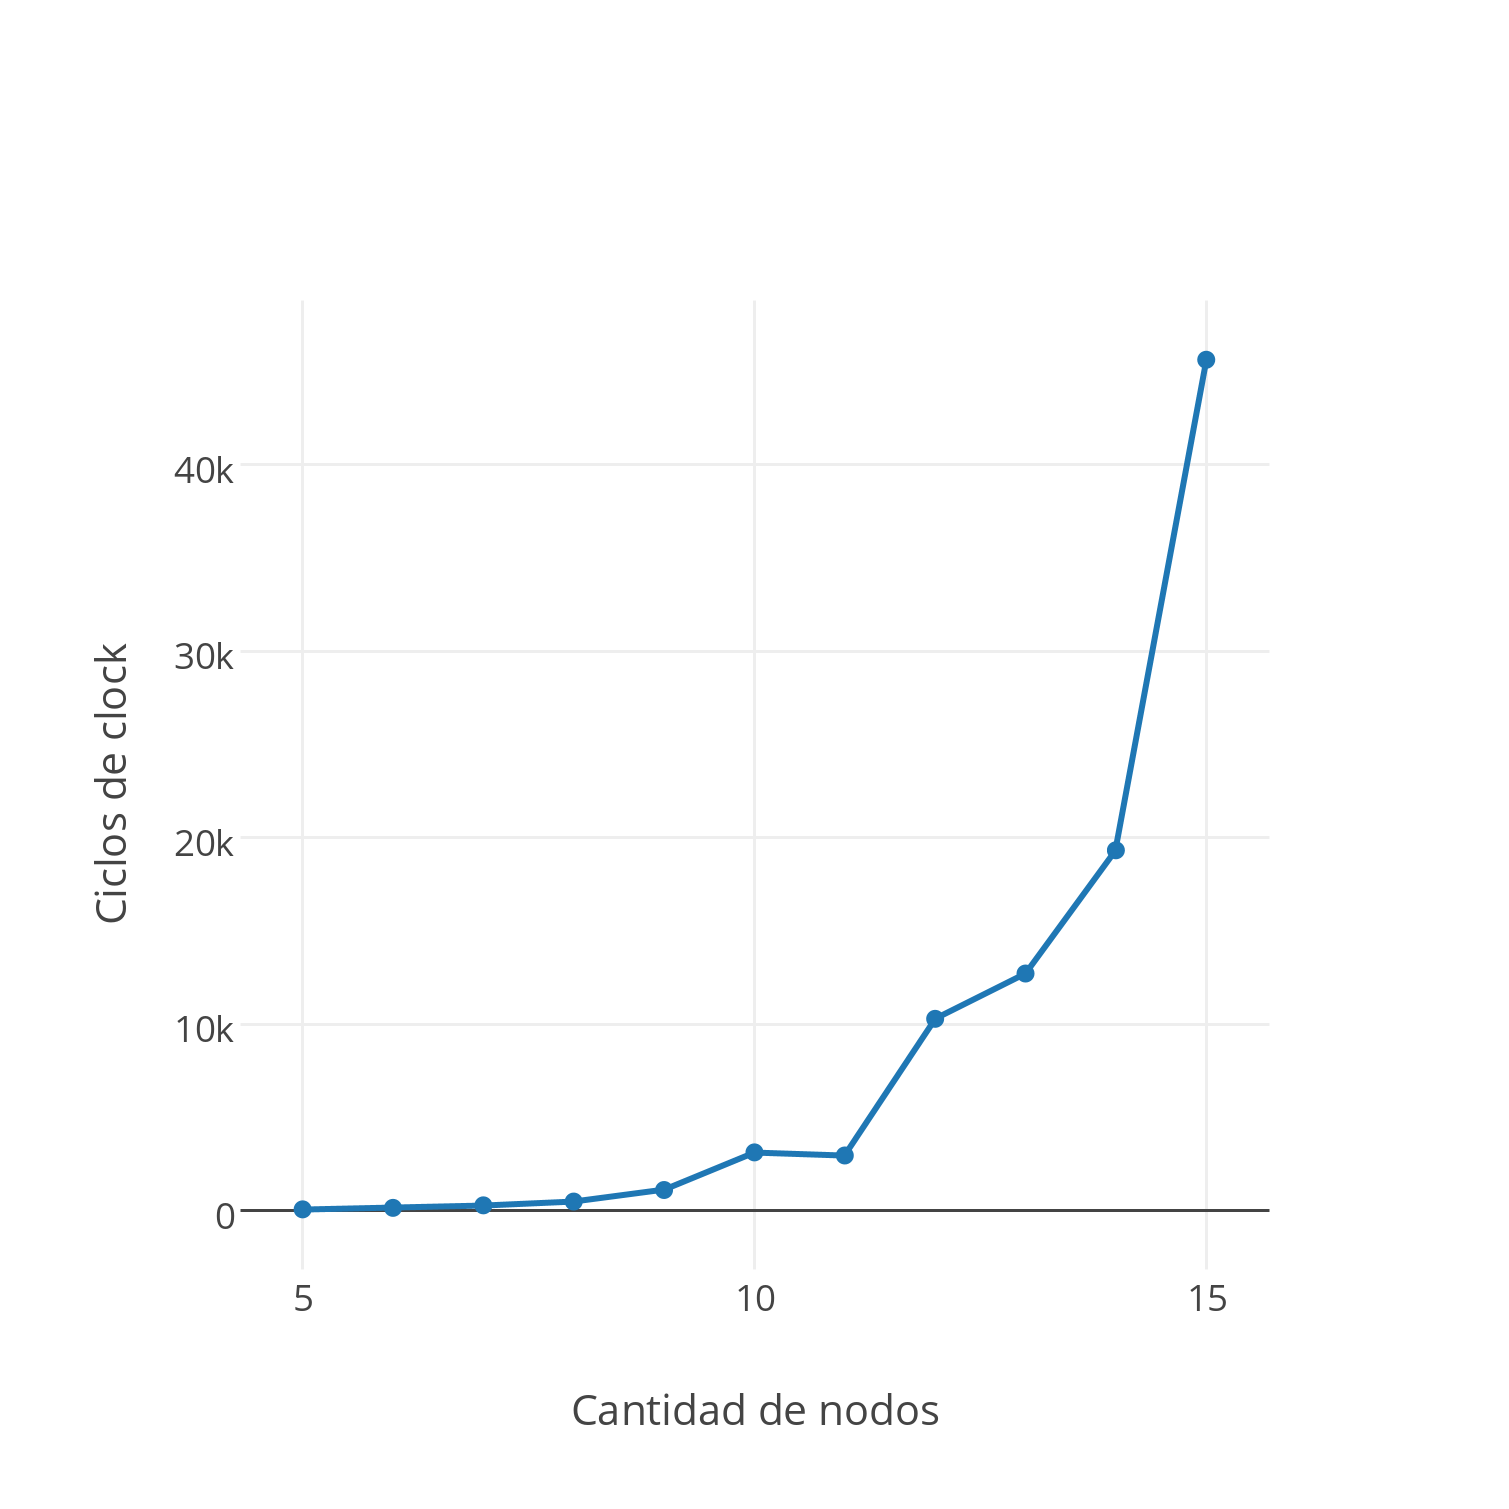
\includegraphics[scale=0.7]{imagenes/exacto-tiempo.png}
\end{center}
  \caption{Exacto - Tiempo de ejecución}\label{fig:1A}
\endminipage\hfill
\minipage{0.5\textwidth}
\begin{center}
  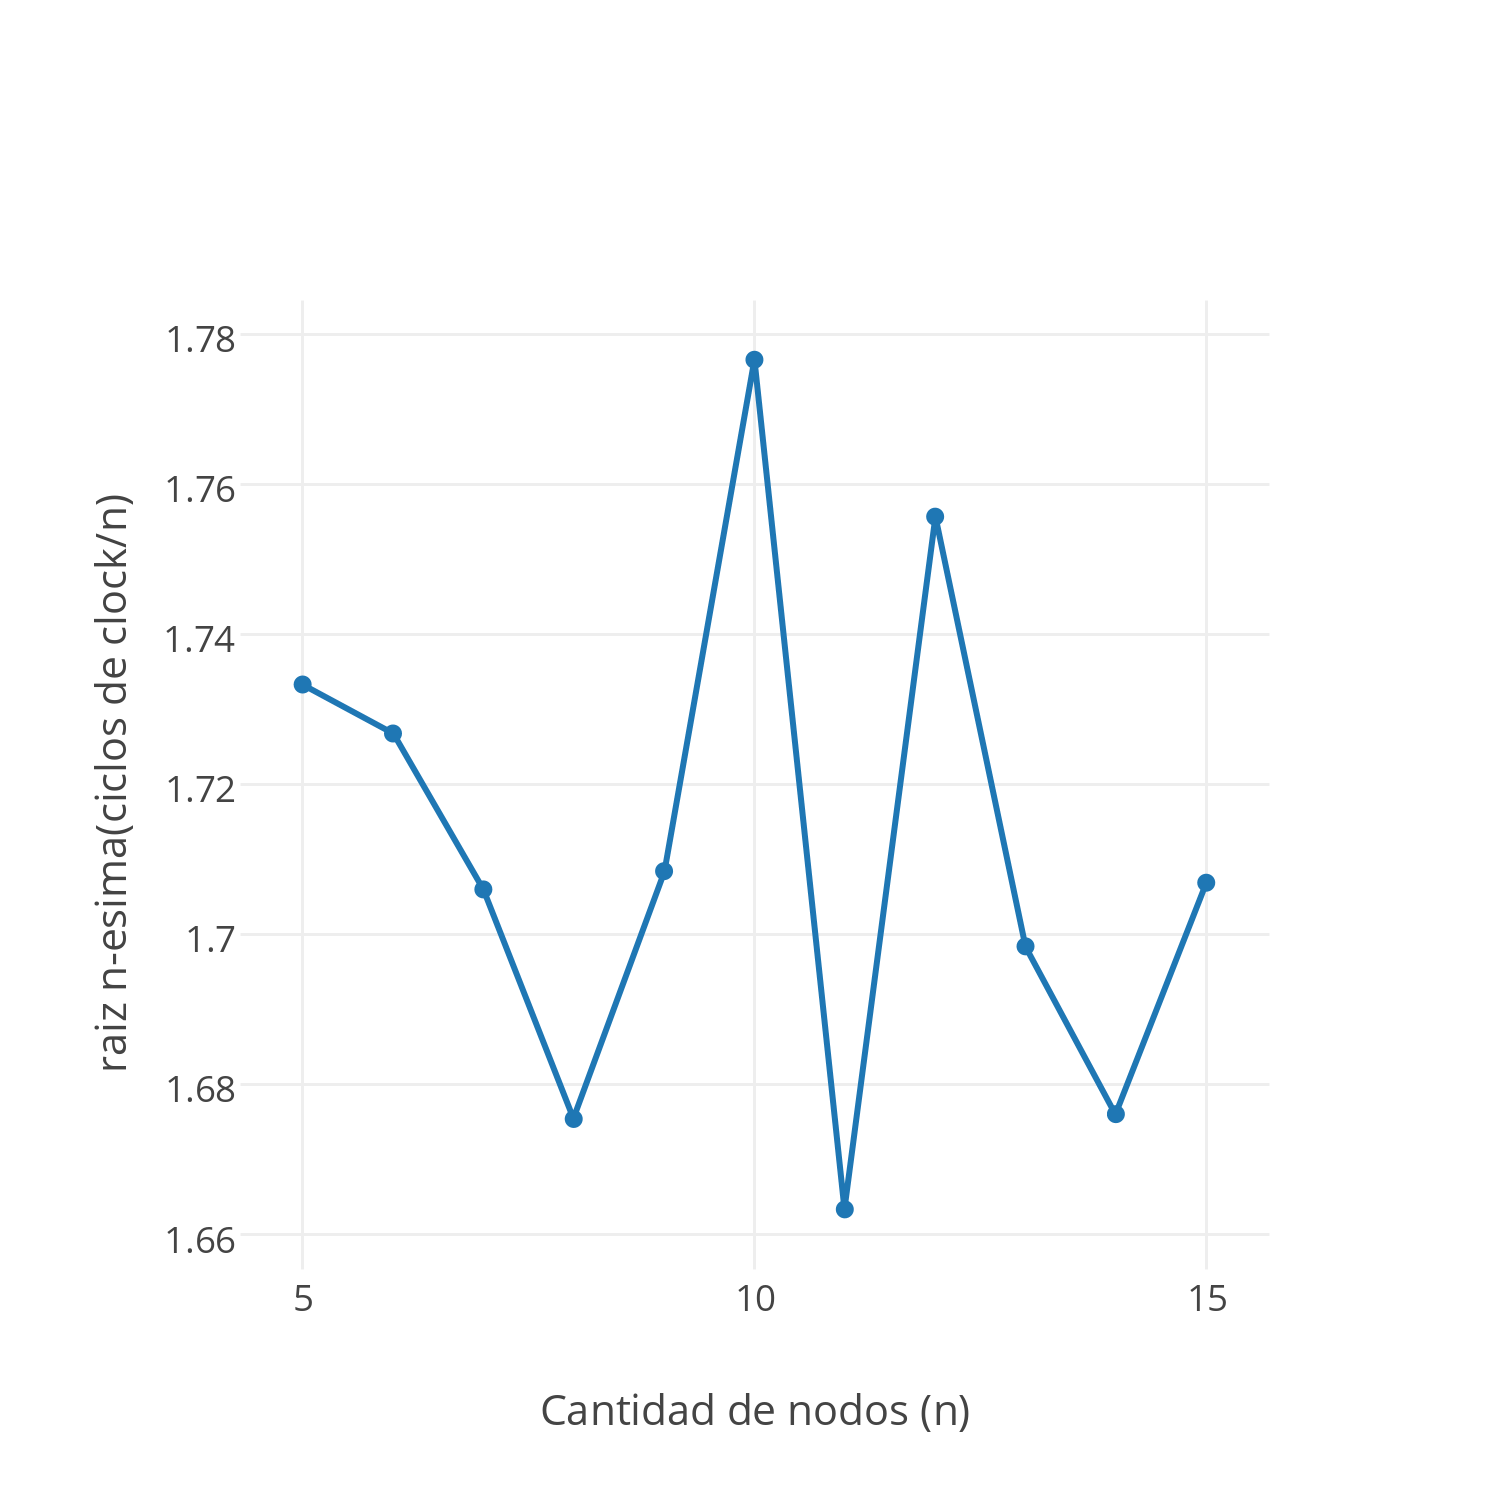
\includegraphics[scale=0.7]{imagenes/exacto-tiempo-raiz.png}
\end{center}
  \caption{Exacto - Tiempo de ejecución}\label{fig:1B}
\endminipage
\end{figure}

%\newpage

\subsubsection{Podas}

Además de la poda clásica, se han generado dos podas más, llamadas ``nodos solitarios'' y ``nodo decisivo'', explicadas anteriormente. Trataremos de ver en esta sección la utilidad de las mismas. Para ello veremos cómo repercuten estas podas en algunas familias de grafos, y tomaremos las instancias $aleatorias$ que usamos para mostrar la complejidad, para ver cómo mejoran con cada poda, y con la combinación de varias.

Para ello, cada instancia se ha corrido de 5 maneras:

\begin{enumerate}
	\item Sin ninguna poda
	\item Con todas las podas 
	\item Con la poda Clásica
	\item Con la poda Clásica y la poda de los nodos solitarios
	\item Con la poda Clásica y la poda del nodo decisivo
\end{enumerate}

Los experimentos propuestos son los siguientes:

\paragraph{Grafo compuesto por nodos de grado 0}

Se han creado 18 instancias, con grafos que tienen de 3 a 20 nodos, todos de grado 0. 

\subparagraph{Hipótesis} Dadas las características de estos grafos, esperamos ver en los resultados que la poda de los {\it nodos solitarios} tiene mayor impacto en la eficiencia que las demás.

\vspace*{0.3cm}

Luego de ejecutar el programa con las instancias mencionadas, el gráfico obtenido con los resultados es el que se muestra en la Figura \ref{fig:1C}.

\begin{figure}[htb]
	\begin{center}
    		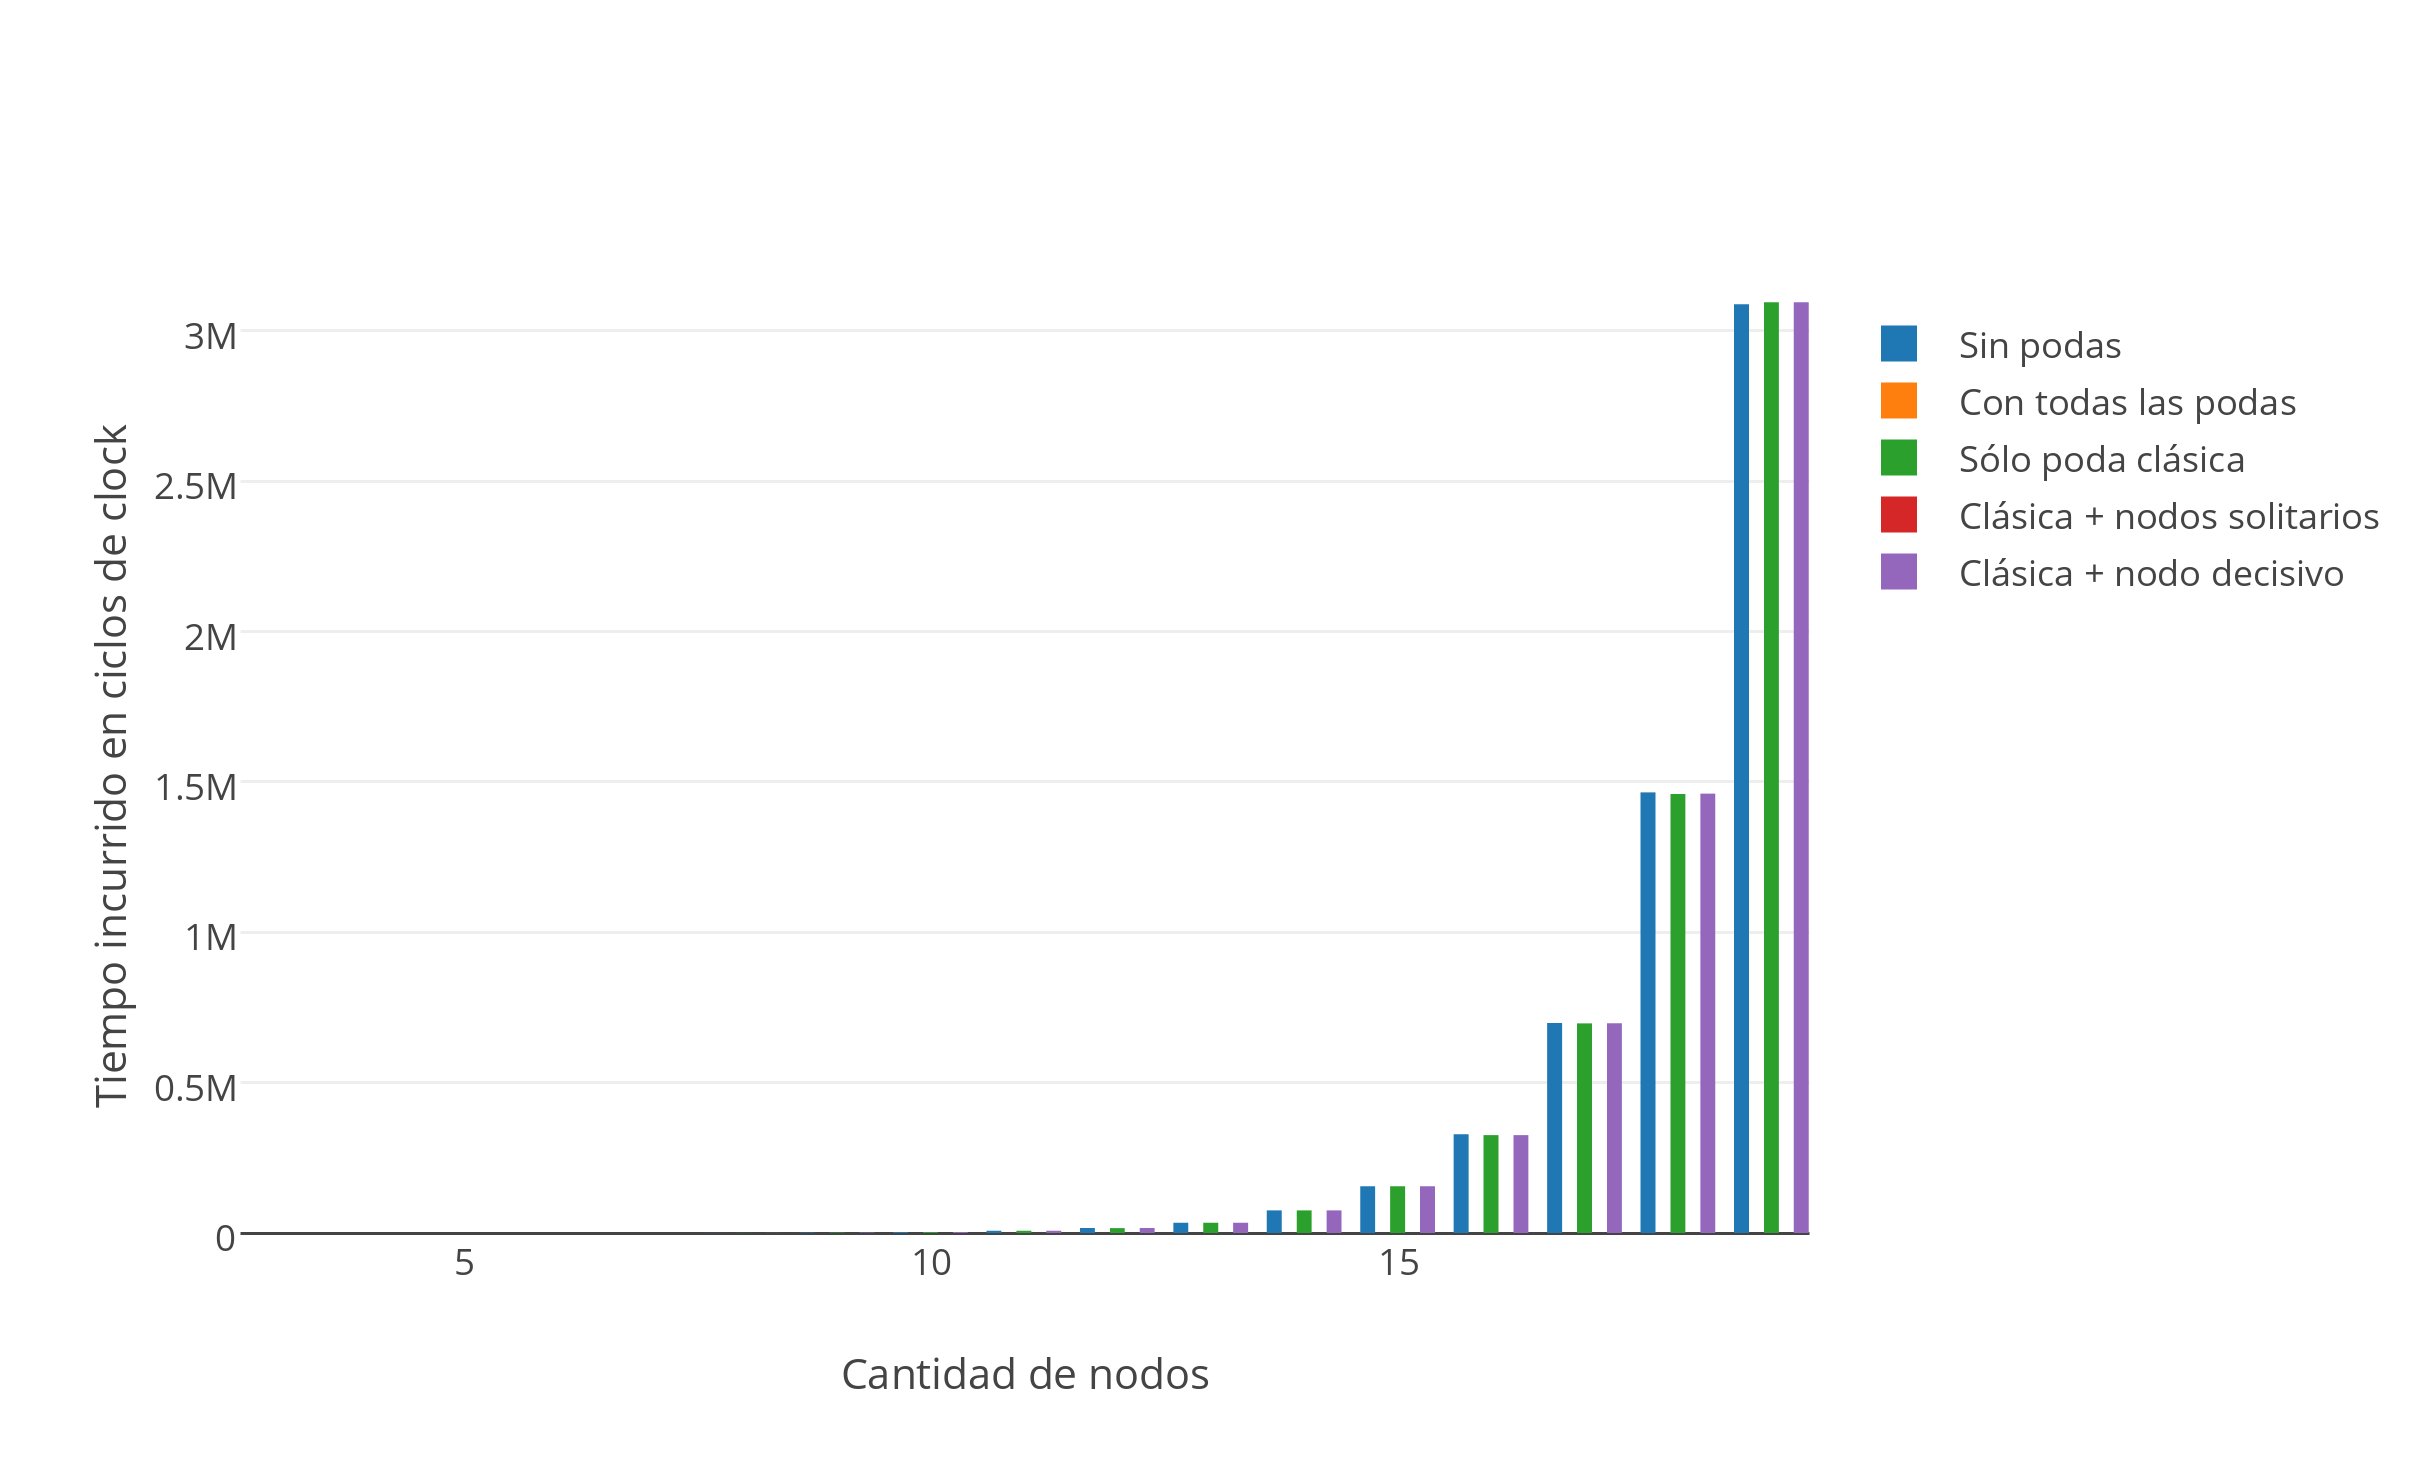
\includegraphics[scale=0.8]{imagenes/exacto-solitarios.png}
	\end{center}
	\caption{Exacto - Nodos solitarios}\label{fig:1C}
\end{figure}
%\FloatBarrier

Por lo visto en este gráfico, la poda de los {\it nodos solitarios} es la que más optimiza el tiempo de ejecución para cuando el grafo está formado por nodos de grado 0.

\paragraph{Grafos completos} 

Se han creado 18 instancias, con grafos completos, de entre 3 y 20 nodos. 

\subparagraph{Hipótesis} Dadas las características de estos grafos, esperamos ver en los resultados que la poda del {\it nodo decisivo} tiene mayor impacto en la eficiencia que las demás.

\vspace*{0.3cm}

El gráfico obtenido con los resultados es el que se muestra en la Figura \ref{fig:1D}.

\begin{figure}[htb]
	\begin{center}
    		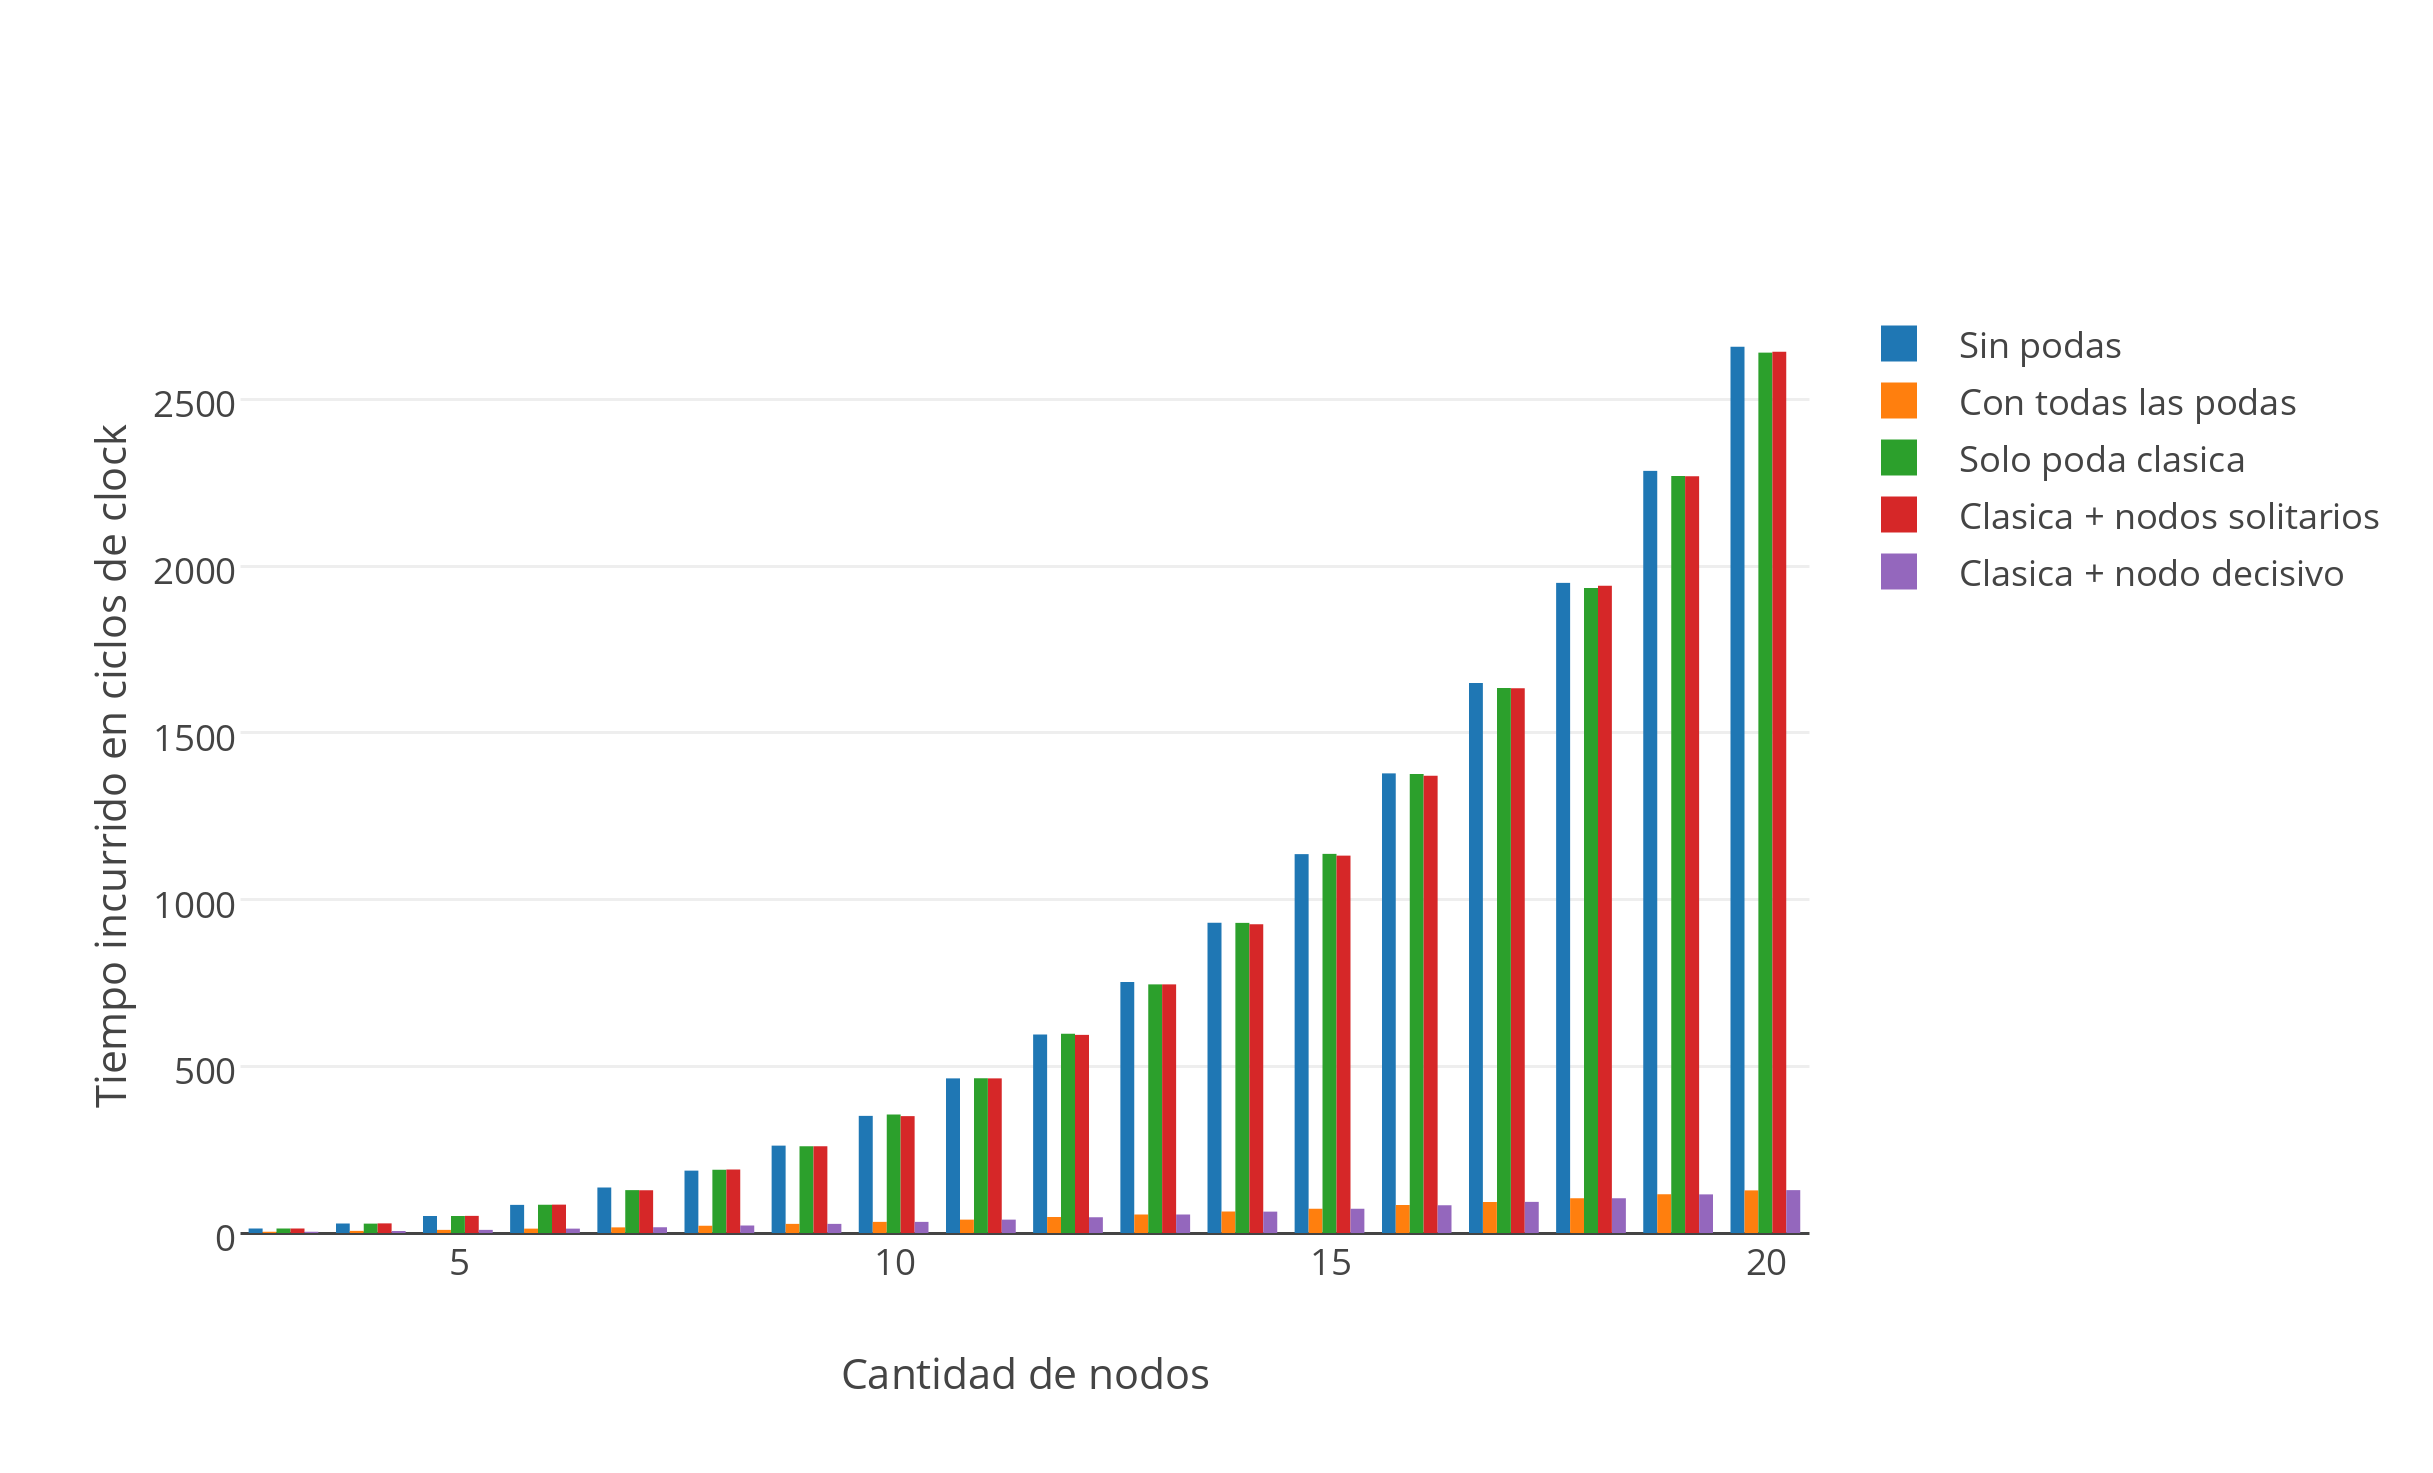
\includegraphics[scale=0.8]{imagenes/exacto-completos.png}
	\end{center}
	\caption{Exacto - Grafos completos}\label{fig:1D}
\end{figure}
%\FloatBarrier

Por lo visto en este gráfico, la poda del {\it nodo decisivo} es la que mayor impacto parece tener en el tiempo de ejecución cuando el grafo tiene nodos de grado máximo.

\paragraph{Grafo compuesto por varios $K_2$}

Se han creado 9 instancias, con grafos compuestos por $n$ $K_2$, con $n$ desde 1 a 9. El orden de los nodos fue aleatorizado para no depender de un rotulado en particular.

\subparagraph{Hipótesis} Esperamos ver en los resultados que ninguna combinación de las podas produce un impacto relevante en la eficiencia, ya que la poda de los {\it nodos solitarios} funciona sólo sobre nodos de grado 0 (que estos grafos no poseen) y la poda del {\it nodo decisivo} funcionará de manera diferente dependiendo el orden en el que se consulten los nodos dentro del programa.

\vspace*{0.3cm}

El gráfico obtenido con los resultados es el que se muestra en la Figura \ref{fig:1E}.

\begin{figure}[htb]
	\begin{center}
    		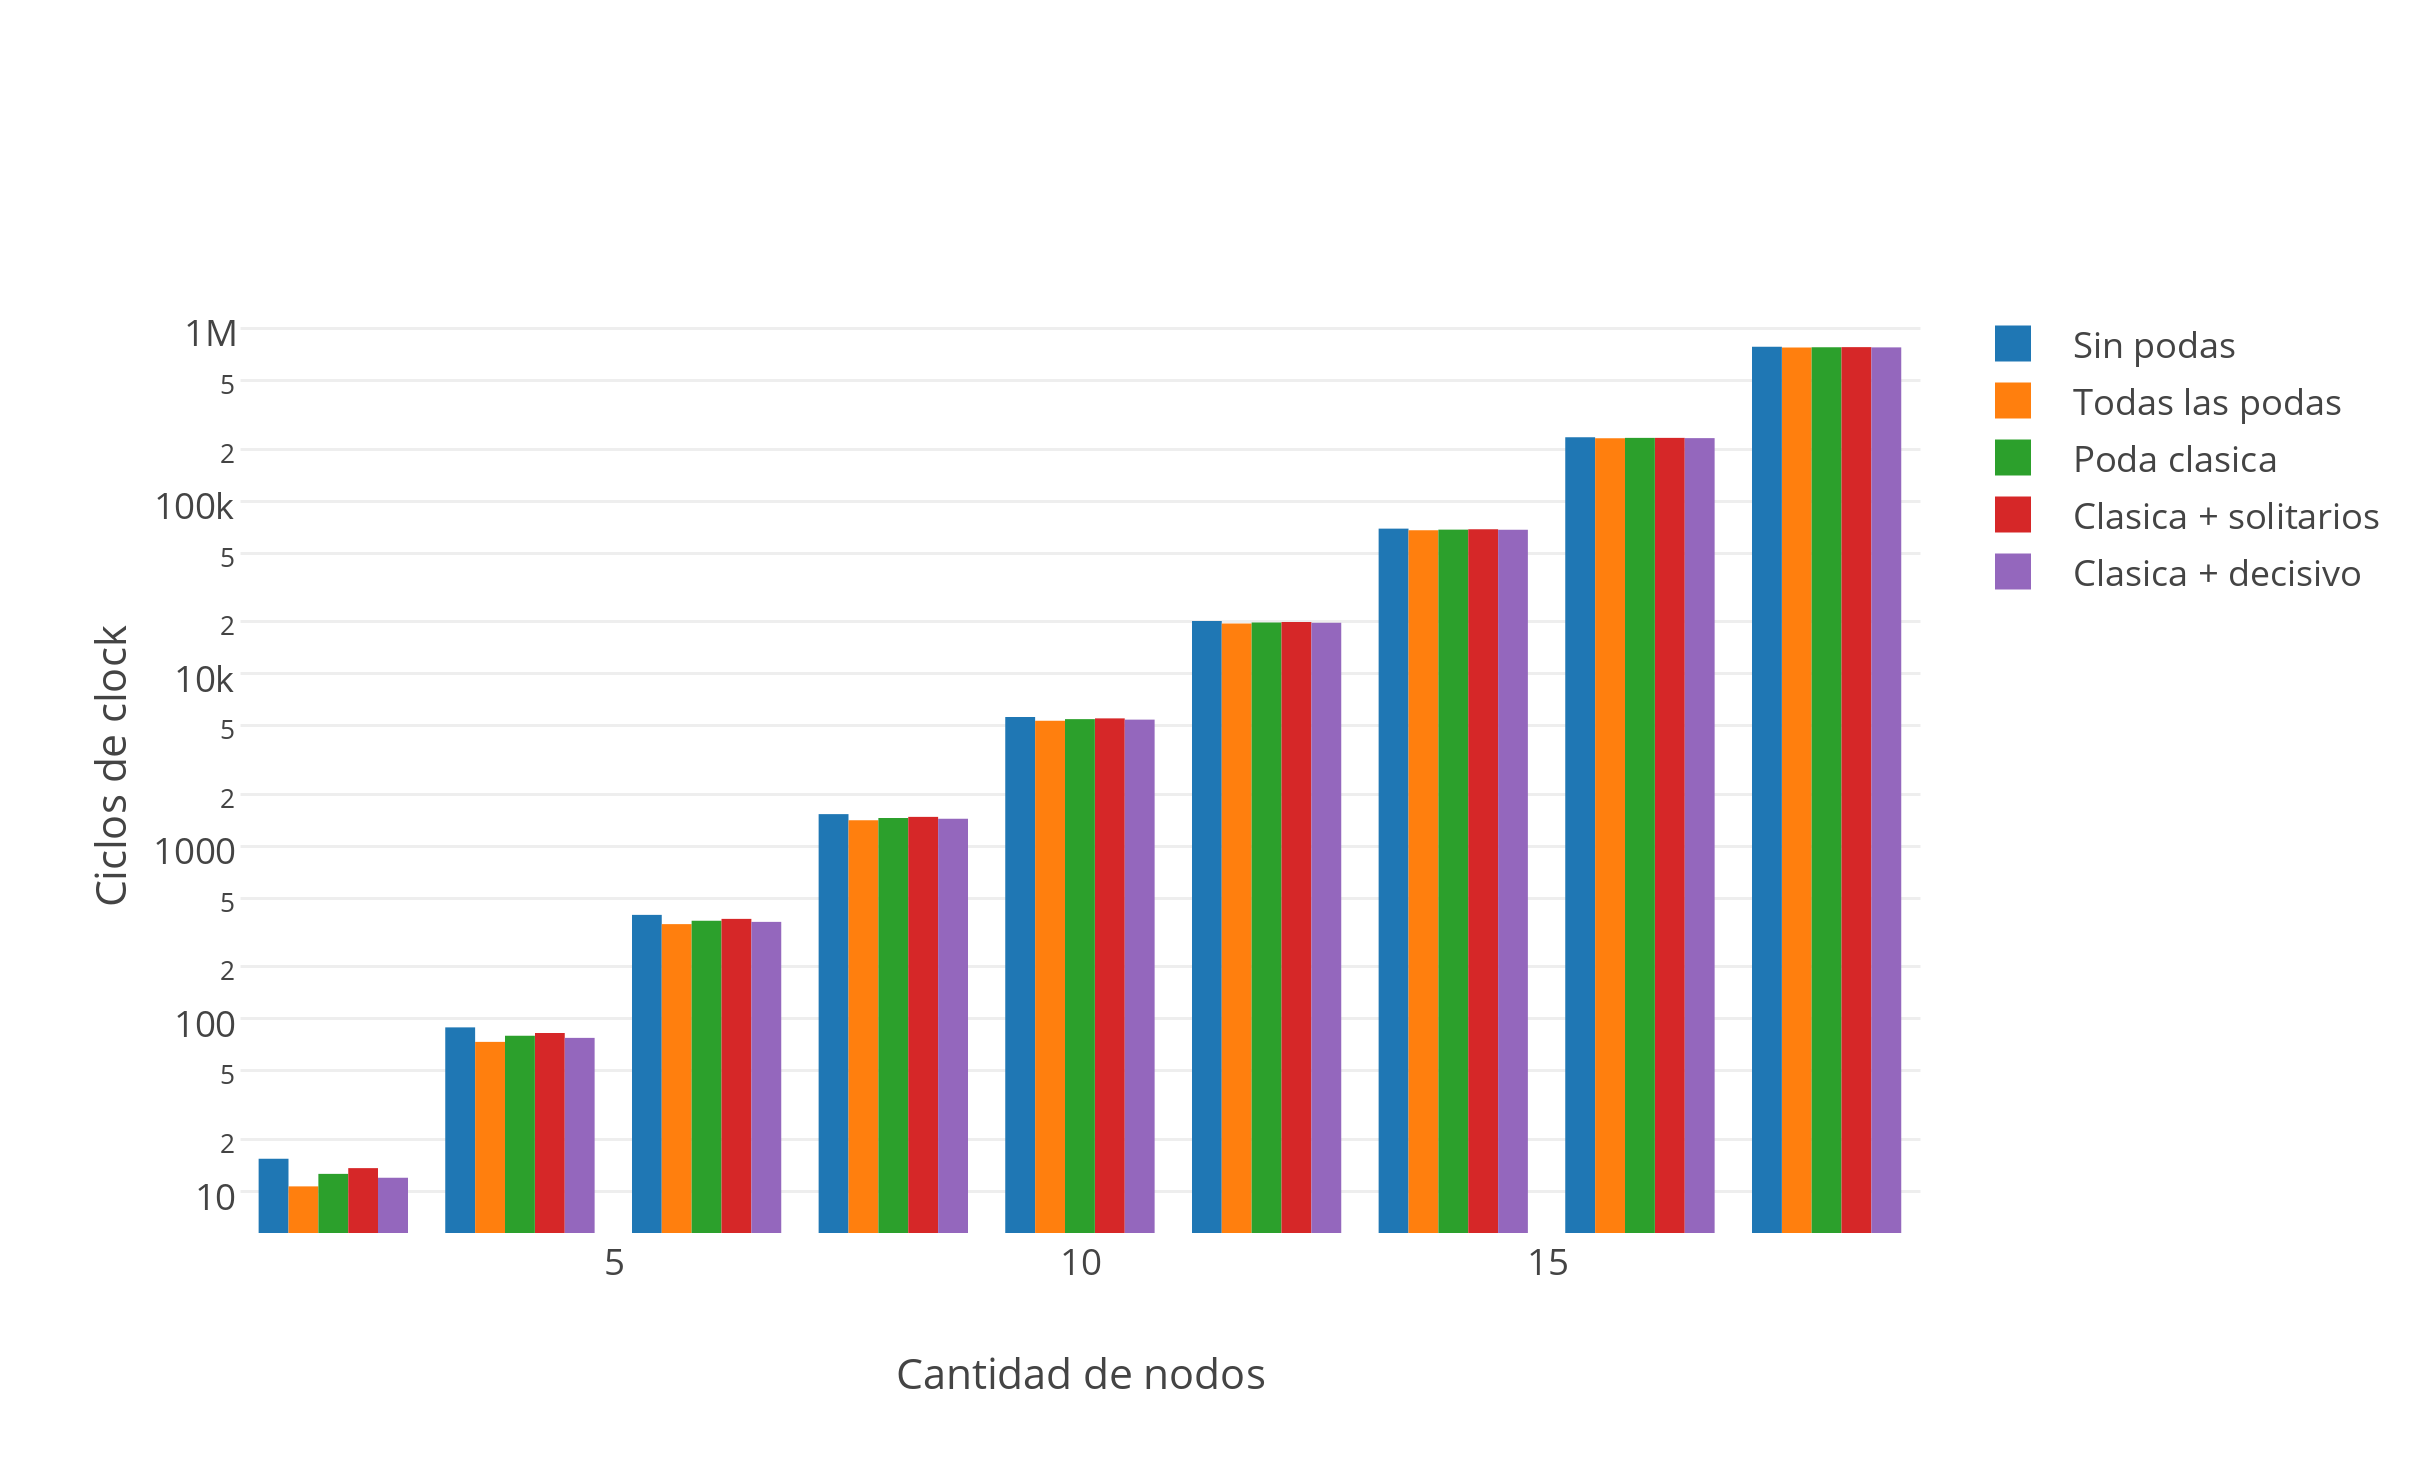
\includegraphics[scale=0.8]{imagenes/exacto-k2.png}
	\end{center}
	\caption{Exacto - Grafos formados por $K_2$}\label{fig:1E}
\end{figure}
%\FloatBarrier

Por lo visto en este gráfico, se trata de una familia en la cual nuestras podas no surten efectos significativos.

\paragraph{Grafos aleatorios}

Se han utilizado las mismas instancias creadas para contrastar la complejidad del algoritmo.

\subparagraph{Hipótesis} Esperamos ver en los resultados que la combinación de todas las podas mejora la performance de manera más significativa que cada poda por separado, ya que considerarlas a todas descarta más ramas de decisión.

\vspace*{0.3cm}

El gráfico obtenido con los resultados es el que se muestra en la Figura \ref{fig:1F}.

\begin{figure}[htb]
	\begin{center}
    		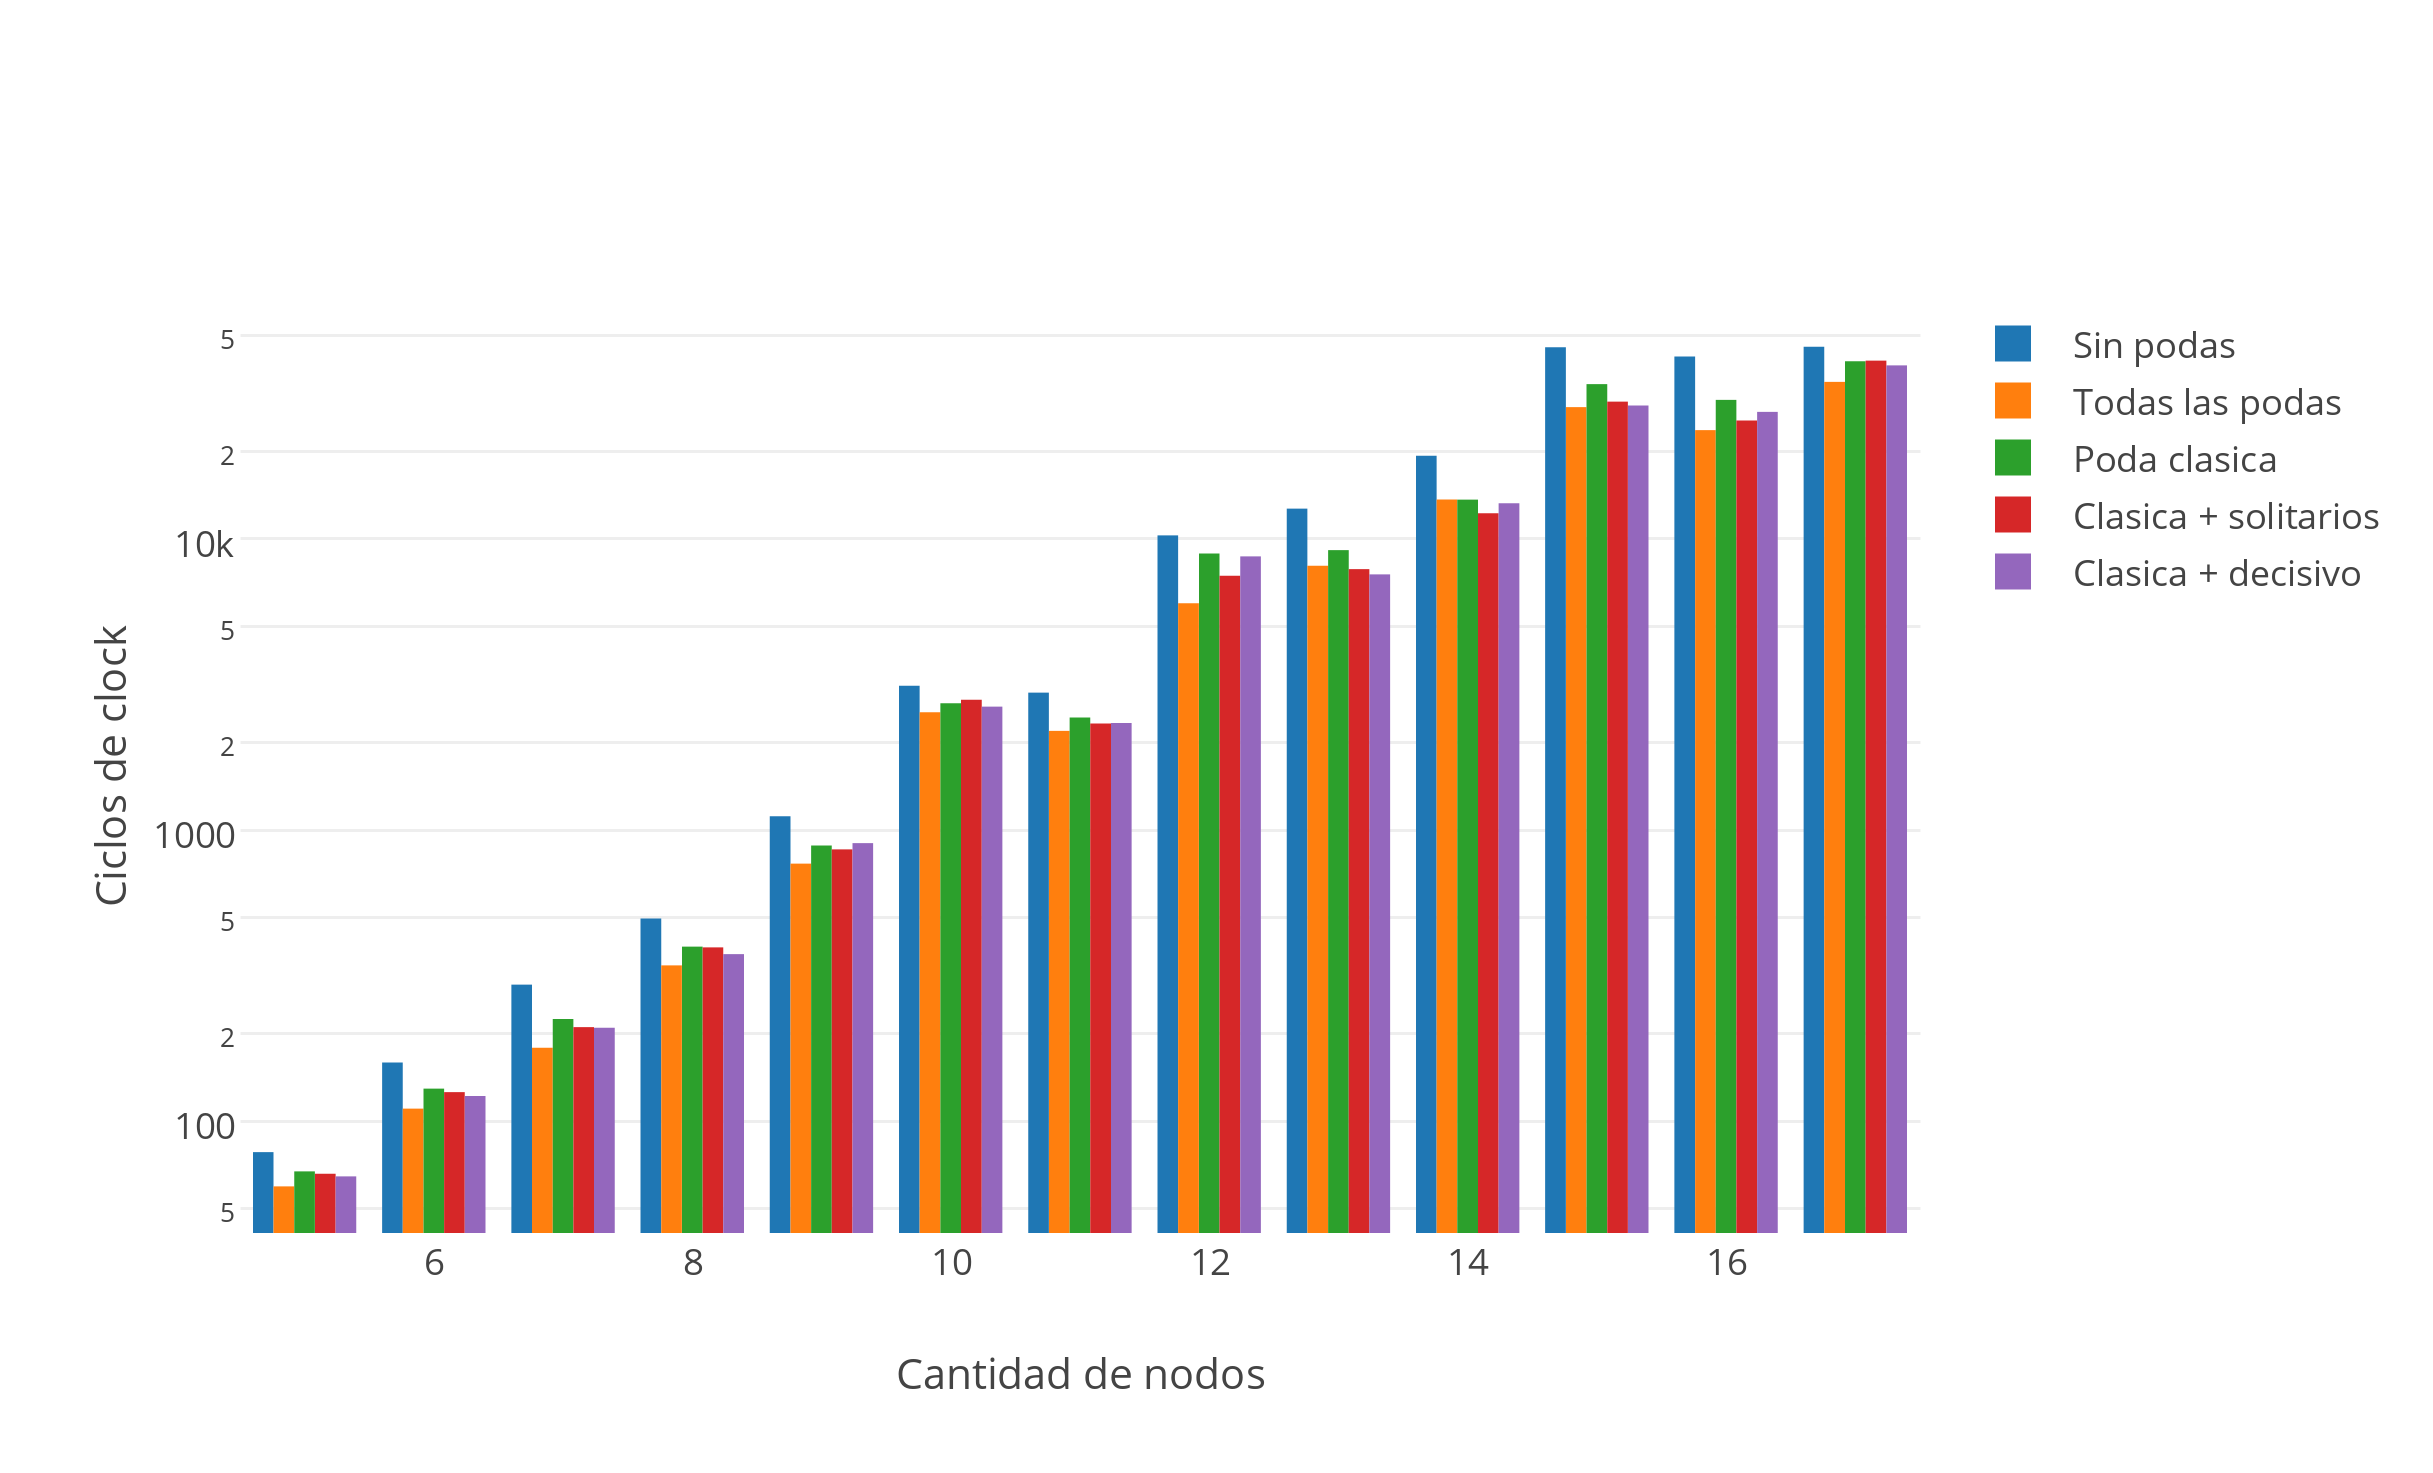
\includegraphics[scale=0.8]{imagenes/exacto-aleatorios.png}
	\end{center}
	\caption{Exacto - Grafos aleatorios\label{fig:1F}}
\end{figure}
%\FloatBarrier

Por lo visto en este gráfico, en general, parecería que usar todas las podas mejora el tiempo de ejecución de nuestro algoritmo, más que utilizar las podas por separado.